\documentclass[1p]{elsarticle_modified}
%\bibliographystyle{elsarticle-num}

%\usepackage[colorlinks]{hyperref}
%\usepackage{abbrmath_seonhwa} %\Abb, \Ascr, \Acal ,\Abf, \Afrak
\usepackage{amsfonts}
\usepackage{amssymb}
\usepackage{amsmath}
\usepackage{amsthm}
\usepackage{scalefnt}
\usepackage{amsbsy}
\usepackage{kotex}
\usepackage{caption}
\usepackage{subfig}
\usepackage{color}
\usepackage{graphicx}
\usepackage{xcolor} %% white, black, red, green, blue, cyan, magenta, yellow
\usepackage{float}
\usepackage{setspace}
\usepackage{hyperref}

\usepackage{tikz}
\usetikzlibrary{arrows}

\usepackage{multirow}
\usepackage{array} % fixed length table
\usepackage{hhline}

%%%%%%%%%%%%%%%%%%%%%
\makeatletter
\renewcommand*\env@matrix[1][\arraystretch]{%
	\edef\arraystretch{#1}%
	\hskip -\arraycolsep
	\let\@ifnextchar\new@ifnextchar
	\array{*\c@MaxMatrixCols c}}
\makeatother %https://tex.stackexchange.com/questions/14071/how-can-i-increase-the-line-spacing-in-a-matrix
%%%%%%%%%%%%%%%

\usepackage[normalem]{ulem}

\newcommand{\msout}[1]{\ifmmode\text{\sout{\ensuremath{#1}}}\else\sout{#1}\fi}
%SOURCE: \msout is \stkout macro in https://tex.stackexchange.com/questions/20609/strikeout-in-math-mode

\newcommand{\cancel}[1]{
	\ifmmode
	{\color{red}\msout{#1}}
	\else
	{\color{red}\sout{#1}}
	\fi
}

\newcommand{\add}[1]{
	{\color{blue}\uwave{#1}}
}

\newcommand{\replace}[2]{
	\ifmmode
	{\color{red}\msout{#1}}{\color{blue}\uwave{#2}}
	\else
	{\color{red}\sout{#1}}{\color{blue}\uwave{#2}}
	\fi
}

\newcommand{\Sol}{\mathcal{S}} %segment
\newcommand{\D}{D} %diagram
\newcommand{\A}{\mathcal{A}} %arc


%%%%%%%%%%%%%%%%%%%%%%%%%%%%%5 test

\def\sl{\operatorname{\textup{SL}}(2,\Cbb)}
\def\psl{\operatorname{\textup{PSL}}(2,\Cbb)}
\def\quan{\mkern 1mu \triangleright \mkern 1mu}

\theoremstyle{definition}
\newtheorem{thm}{Theorem}[section]
\newtheorem{prop}[thm]{Proposition}
\newtheorem{lem}[thm]{Lemma}
\newtheorem{ques}[thm]{Question}
\newtheorem{cor}[thm]{Corollary}
\newtheorem{defn}[thm]{Definition}
\newtheorem{exam}[thm]{Example}
\newtheorem{rmk}[thm]{Remark}
\newtheorem{alg}[thm]{Algorithm}

\newcommand{\I}{\sqrt{-1}}
\begin{document}

%\begin{frontmatter}
%
%\title{Boundary parabolic representations of knots up to 8 crossings}
%
%%% Group authors per affiliation:
%\author{Yunhi Cho} 
%\address{Department of Mathematics, University of Seoul, Seoul, Korea}
%\ead{yhcho@uos.ac.kr}
%
%
%\author{Seonhwa Kim} %\fnref{s_kim}}
%\address{Center for Geometry and Physics, Institute for Basic Science, Pohang, 37673, Korea}
%\ead{ryeona17@ibs.re.kr}
%
%\author{Hyuk Kim}
%\address{Department of Mathematical Sciences, Seoul National University, Seoul 08826, Korea}
%\ead{hyukkim@snu.ac.kr}
%
%\author{Seokbeom Yoon}
%\address{Department of Mathematical Sciences, Seoul National University, Seoul, 08826,  Korea}
%\ead{sbyoon15@snu.ac.kr}
%
%\begin{abstract}
%We find all boundary parabolic representation of knots up to 8 crossings.
%
%\end{abstract}
%\begin{keyword}
%    \MSC[2010] 57M25 
%\end{keyword}
%
%\end{frontmatter}

%\linenumbers
%\tableofcontents
%
\newcommand\colored[1]{\textcolor{white}{\rule[-0.35ex]{0.8em}{1.4ex}}\kern-0.8em\color{red} #1}%
%\newcommand\colored[1]{\textcolor{white}{ #1}\kern-2.17ex	\textcolor{white}{ #1}\kern-1.81ex	\textcolor{white}{ #1}\kern-2.15ex\color{red}#1	}

{\Large $\underline{11n_{65}~(K11n_{65})}$}

\setlength{\tabcolsep}{10pt}
\renewcommand{\arraystretch}{1.6}
\vspace{1cm}\begin{tabular}{m{100pt}>{\centering\arraybackslash}m{274pt}}
\multirow{5}{120pt}{
	\centering
	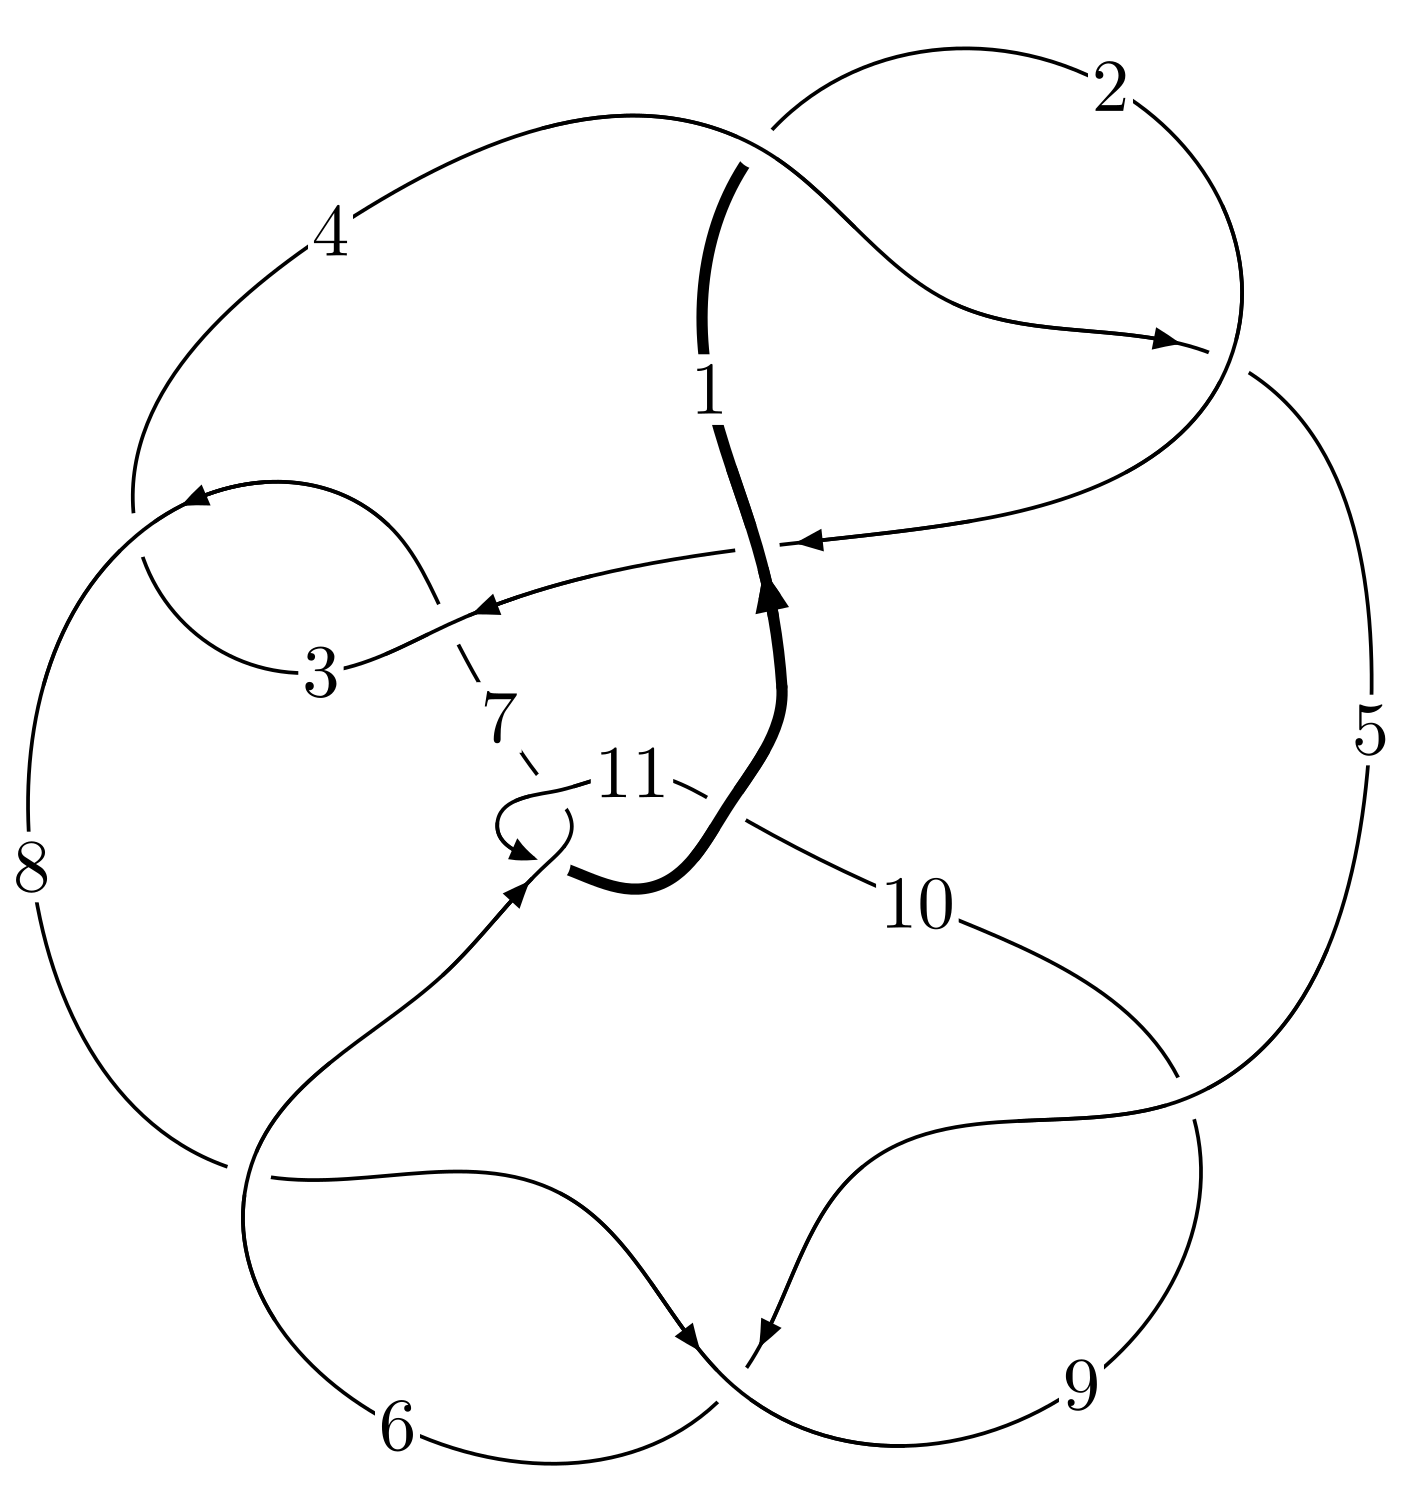
\includegraphics[width=112pt]{../../../GIT/diagram.site/Diagrams/png/681_11n_65.png}\\
\ \ \ A knot diagram\footnotemark}&
\allowdisplaybreaks
\textbf{Linearized knot diagam} \\
\cline{2-2}
 &
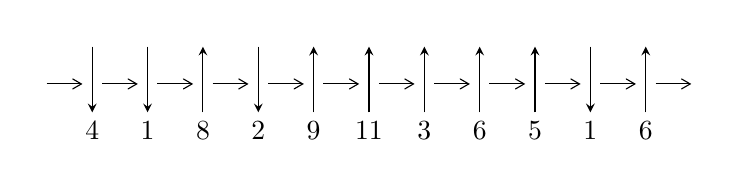
\begin{tikzpicture}[x=20pt, y=17pt]
	% nodes
	\node (C0) at (0, 0) {};
	\node (C1) at (1, 0) {};
	\node (C1U) at (1, +1) {};
	\node (C1D) at (1, -1) {4};

	\node (C2) at (2, 0) {};
	\node (C2U) at (2, +1) {};
	\node (C2D) at (2, -1) {1};

	\node (C3) at (3, 0) {};
	\node (C3U) at (3, +1) {};
	\node (C3D) at (3, -1) {8};

	\node (C4) at (4, 0) {};
	\node (C4U) at (4, +1) {};
	\node (C4D) at (4, -1) {2};

	\node (C5) at (5, 0) {};
	\node (C5U) at (5, +1) {};
	\node (C5D) at (5, -1) {9};

	\node (C6) at (6, 0) {};
	\node (C6U) at (6, +1) {};
	\node (C6D) at (6, -1) {11};

	\node (C7) at (7, 0) {};
	\node (C7U) at (7, +1) {};
	\node (C7D) at (7, -1) {3};

	\node (C8) at (8, 0) {};
	\node (C8U) at (8, +1) {};
	\node (C8D) at (8, -1) {6};

	\node (C9) at (9, 0) {};
	\node (C9U) at (9, +1) {};
	\node (C9D) at (9, -1) {5};

	\node (C10) at (10, 0) {};
	\node (C10U) at (10, +1) {};
	\node (C10D) at (10, -1) {1};

	\node (C11) at (11, 0) {};
	\node (C11U) at (11, +1) {};
	\node (C11D) at (11, -1) {6};
	\node (C12) at (12, 0) {};

	% arrows
	\draw[->,>={angle 60}]
	(C0) edge (C1) (C1) edge (C2) (C2) edge (C3) (C3) edge (C4) (C4) edge (C5) (C5) edge (C6) (C6) edge (C7) (C7) edge (C8) (C8) edge (C9) (C9) edge (C10) (C10) edge (C11) (C11) edge (C12) ;	\draw[->,>=stealth]
	(C1U) edge (C1D) (C2U) edge (C2D) (C3D) edge (C3U) (C4U) edge (C4D) (C5D) edge (C5U) (C6D) edge (C6U) (C7D) edge (C7U) (C8D) edge (C8U) (C9D) edge (C9U) (C10U) edge (C10D) (C11D) edge (C11U) ;
	\end{tikzpicture} \\
\hhline{~~} \\& 
\textbf{Solving Sequence} \\ \cline{2-2} 
 &
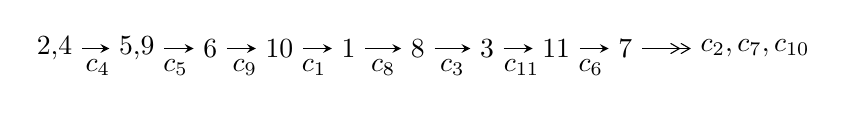
\begin{tikzpicture}[x=25pt, y=7pt]
	% node
	\node (A0) at (-1/8, 0) {2,4};
	\node (A1) at (17/16, 0) {5,9};
	\node (A2) at (17/8, 0) {6};
	\node (A3) at (25/8, 0) {10};
	\node (A4) at (33/8, 0) {1};
	\node (A5) at (41/8, 0) {8};
	\node (A6) at (49/8, 0) {3};
	\node (A7) at (57/8, 0) {11};
	\node (A8) at (65/8, 0) {7};
	\node (C1) at (1/2, -1) {$c_{4}$};
	\node (C2) at (13/8, -1) {$c_{5}$};
	\node (C3) at (21/8, -1) {$c_{9}$};
	\node (C4) at (29/8, -1) {$c_{1}$};
	\node (C5) at (37/8, -1) {$c_{8}$};
	\node (C6) at (45/8, -1) {$c_{3}$};
	\node (C7) at (53/8, -1) {$c_{11}$};
	\node (C8) at (61/8, -1) {$c_{6}$};
	\node (A9) at (10, 0) {$c_{2},c_{7},c_{10}$};

	% edge
	\draw[->,>=stealth]	
	(A0) edge (A1) (A1) edge (A2) (A2) edge (A3) (A3) edge (A4) (A4) edge (A5) (A5) edge (A6) (A6) edge (A7) (A7) edge (A8) ;
	\draw[->>,>={angle 60}]	
	(A8) edge (A9);
\end{tikzpicture} \\ 

\end{tabular} \\

\footnotetext{
The image of knot diagram is generated by the software ``\textbf{Draw programme}" developed by Andrew Bartholomew(\url{http://www.layer8.co.uk/maths/draw/index.htm\#Running-draw}), where we modified some parts for our purpose(\url{https://github.com/CATsTAILs/LinksPainter}).
}\phantom \\ \newline 
\centering \textbf{Ideals for irreducible components\footnotemark of $X_{\text{par}}$} 
 
\begin{align*}
I^u_{1}&=\langle 
2666 u^{12}-2811 u^{11}+\cdots+9382 b+3250,\;-1563 u^{12}+2980 u^{11}+\cdots+18764 a+7547,\\
\phantom{I^u_{1}}&\phantom{= \langle  }u^{13}-2 u^{12}-2 u^{11}+7 u^{10}- u^9-9 u^8+16 u^7-18 u^6-2 u^5+33 u^4-24 u^3-10 u^2+17 u-4\rangle \\
I^u_{2}&=\langle 
- u^4+u^3+2 u^2+b- a- u-1,\;u^4-2 u^2 a-2 u^3+a^2+a u+2 a+u+2,\;u^5- u^4-2 u^3+u^2+u+1\rangle \\
I^u_{3}&=\langle 
- u^2 a+a u- u^2+b+u-1,\;2 u^2 a+a^2-4 a u+3 u^2+2 a-6 u+5,\;u^3- u^2+1\rangle \\
I^u_{4}&=\langle 
2 b+1,\;2 a-1,\;u+1\rangle \\
\\
\end{align*}
\raggedright * 4 irreducible components of $\dim_{\mathbb{C}}=0$, with total 30 representations.\\
\footnotetext{All coefficients of polynomials are rational numbers. But the coefficients are sometimes approximated in decimal forms when there is not enough margin.}
\newpage
\renewcommand{\arraystretch}{1}
\centering \section*{I. $I^u_{1}= \langle 2666 u^{12}-2811 u^{11}+\cdots+9382 b+3250,\;-1563 u^{12}+2980 u^{11}+\cdots+18764 a+7547,\;u^{13}-2 u^{12}+\cdots+17 u-4 \rangle$}
\flushleft \textbf{(i) Arc colorings}\\
\begin{tabular}{m{7pt} m{180pt} m{7pt} m{180pt} }
\flushright $a_{2}=$&$\begin{pmatrix}0\\u\end{pmatrix}$ \\
\flushright $a_{4}=$&$\begin{pmatrix}1\\0\end{pmatrix}$ \\
\flushright $a_{5}=$&$\begin{pmatrix}1\\u^2\end{pmatrix}$ \\
\flushright $a_{9}=$&$\begin{pmatrix}0.0832978 u^{12}-0.158815 u^{11}+\cdots-2.36613 u-0.402206\\-0.284161 u^{12}+0.299616 u^{11}+\cdots+3.21925 u-0.346408\end{pmatrix}$ \\
\flushright $a_{6}=$&$\begin{pmatrix}-0.0329887 u^{12}+0.0405031 u^{11}+\cdots+0.801428 u+1.42640\\0.0613942 u^{12}-0.0681091 u^{11}+\cdots-0.833191 u+0.0125773\end{pmatrix}$ \\
\flushright $a_{10}=$&$\begin{pmatrix}0.00314432 u^{12}+0.0551055 u^{11}+\cdots+0.652206 u-0.779738\\-0.0254743 u^{12}+0.129823 u^{11}+\cdots+1.98721 u-0.131955\end{pmatrix}$ \\
\flushright $a_{1}=$&$\begin{pmatrix}u\\u\end{pmatrix}$ \\
\flushright $a_{8}=$&$\begin{pmatrix}-0.0853763 u^{12}-0.131848 u^{11}+\cdots-2.30228 u-1.25187\\-0.481454 u^{12}+0.401300 u^{11}+\cdots+4.61810 u-0.548284\end{pmatrix}$ \\
\flushright $a_{3}=$&$\begin{pmatrix}- u^3\\- u^3+u\end{pmatrix}$ \\
\flushright $a_{11}=$&$\begin{pmatrix}-0.168674 u^{12}+0.0269665 u^{11}+\cdots+1.06385 u-0.849659\\-0.197293 u^{12}+0.101684 u^{11}+\cdots+2.39885 u-0.201876\end{pmatrix}$ \\
\flushright $a_{7}=$&$\begin{pmatrix}0.334683 u^{12}-0.465039 u^{11}+\cdots-4.08719 u+3.28384\\0.169154 u^{12}-0.382967 u^{11}+\cdots-3.37114 u+0.654445\end{pmatrix}$\\ \flushright $a_{7}=$&$\begin{pmatrix}0.334683 u^{12}-0.465039 u^{11}+\cdots-4.08719 u+3.28384\\0.169154 u^{12}-0.382967 u^{11}+\cdots-3.37114 u+0.654445\end{pmatrix}$\\&\end{tabular}
\flushleft \textbf{(ii) Obstruction class $= -1$}\\~\\
\flushleft \textbf{(iii) Cusp Shapes $= \frac{34825}{18764} u^{12}-\frac{68759}{18764} u^{11}+\cdots-\frac{496503}{18764} u+\frac{97945}{4691}$}\\~\\
\newpage\renewcommand{\arraystretch}{1}
\flushleft \textbf{(iv) u-Polynomials at the component}\newline \\
\begin{tabular}{m{50pt}|m{274pt}}
Crossings & \hspace{64pt}u-Polynomials at each crossing \\
\hline $$\begin{aligned}c_{1},c_{4}\end{aligned}$$&$\begin{aligned}
&u^{13}-2 u^{12}+\cdots+17 u-4
\end{aligned}$\\
\hline $$\begin{aligned}c_{2}\end{aligned}$$&$\begin{aligned}
&u^{13}+8 u^{12}+\cdots+209 u+16
\end{aligned}$\\
\hline $$\begin{aligned}c_{3},c_{7}\end{aligned}$$&$\begin{aligned}
&u^{13}+3 u^{12}+\cdots-2 u-8
\end{aligned}$\\
\hline $$\begin{aligned}c_{5},c_{6},c_{8}\\c_{9},c_{11}\end{aligned}$$&$\begin{aligned}
&u^{13}- u^{12}+\cdots+u-1
\end{aligned}$\\
\hline $$\begin{aligned}c_{10}\end{aligned}$$&$\begin{aligned}
&u^{13}+19 u^{12}+\cdots-13 u-1
\end{aligned}$\\
\hline
\end{tabular}\\~\\
\newpage\renewcommand{\arraystretch}{1}
\flushleft \textbf{(v) Riley Polynomials at the component}\newline \\
\begin{tabular}{m{50pt}|m{274pt}}
Crossings & \hspace{64pt}Riley Polynomials at each crossing \\
\hline $$\begin{aligned}c_{1},c_{4}\end{aligned}$$&$\begin{aligned}
&y^{13}-8 y^{12}+\cdots+209 y-16
\end{aligned}$\\
\hline $$\begin{aligned}c_{2}\end{aligned}$$&$\begin{aligned}
&y^{13}-4 y^{12}+\cdots+22817 y-256
\end{aligned}$\\
\hline $$\begin{aligned}c_{3},c_{7}\end{aligned}$$&$\begin{aligned}
&y^{13}-3 y^{12}+\cdots+180 y-64
\end{aligned}$\\
\hline $$\begin{aligned}c_{5},c_{6},c_{8}\\c_{9},c_{11}\end{aligned}$$&$\begin{aligned}
&y^{13}+19 y^{12}+\cdots-13 y-1
\end{aligned}$\\
\hline $$\begin{aligned}c_{10}\end{aligned}$$&$\begin{aligned}
&y^{13}-49 y^{12}+\cdots-61 y-1
\end{aligned}$\\
\hline
\end{tabular}\\~\\
\newpage\flushleft \textbf{(vi) Complex Volumes and Cusp Shapes}
$$\begin{array}{c|c|c}  
\text{Solutions to }I^u_{1}& \I (\text{vol} + \sqrt{-1}CS) & \text{Cusp shape}\\
 \hline 
\begin{aligned}
u &= \phantom{-}0.955186 + 0.433947 I \\
a &= -0.471198 - 0.436221 I \\
b &= \phantom{-}0.755123 - 0.031476 I\end{aligned}
 & \phantom{-}0.903643 - 0.585016 I & \phantom{-}4.40140 + 1.35233 I \\ \hline\begin{aligned}
u &= \phantom{-}0.955186 - 0.433947 I \\
a &= -0.471198 + 0.436221 I \\
b &= \phantom{-}0.755123 + 0.031476 I\end{aligned}
 & \phantom{-}0.903643 + 0.585016 I & \phantom{-}4.40140 - 1.35233 I \\ \hline\begin{aligned}
u &= -0.933504 + 0.177892 I \\
a &= -0.617558 + 0.567691 I \\
b &= -0.473971 + 0.403774 I\end{aligned}
 & -1.65953 + 0.62739 I & -3.40176 - 1.52650 I \\ \hline\begin{aligned}
u &= -0.933504 - 0.177892 I \\
a &= -0.617558 - 0.567691 I \\
b &= -0.473971 - 0.403774 I\end{aligned}
 & -1.65953 - 0.62739 I & -3.40176 + 1.52650 I \\ \hline\begin{aligned}
u &= \phantom{-}0.869334 + 0.624757 I \\
a &= \phantom{-}0.420041 + 0.925939 I \\
b &= -0.581132 + 0.140274 I\end{aligned}
 & \phantom{-}1.00399 - 3.84064 I & \phantom{-}5.54977 + 8.01840 I \\ \hline\begin{aligned}
u &= \phantom{-}0.869334 - 0.624757 I \\
a &= \phantom{-}0.420041 - 0.925939 I \\
b &= -0.581132 - 0.140274 I\end{aligned}
 & \phantom{-}1.00399 + 3.84064 I & \phantom{-}5.54977 - 8.01840 I \\ \hline\begin{aligned}
u &= -0.028967 + 1.273930 I \\
a &= -0.158932 + 0.197003 I \\
b &= \phantom{-}0.05120 - 2.05742 I\end{aligned}
 & -12.48260 + 4.81706 I & -0.19074 - 2.27482 I \\ \hline\begin{aligned}
u &= -0.028967 - 1.273930 I \\
a &= -0.158932 - 0.197003 I \\
b &= \phantom{-}0.05120 + 2.05742 I\end{aligned}
 & -12.48260 - 4.81706 I & -0.19074 + 2.27482 I \\ \hline\begin{aligned}
u &= \phantom{-}1.46956 + 0.59251 I \\
a &= -0.85770 - 1.47458 I \\
b &= \phantom{-}0.52077 - 2.38909 I\end{aligned}
 & -17.2166 - 11.4167 I & -1.78764 + 5.02800 I \\ \hline\begin{aligned}
u &= \phantom{-}1.46956 - 0.59251 I \\
a &= -0.85770 + 1.47458 I \\
b &= \phantom{-}0.52077 + 2.38909 I\end{aligned}
 & -17.2166 + 11.4167 I & -1.78764 - 5.02800 I\\
 \hline 
 \end{array}$$\newpage$$\begin{array}{c|c|c}  
\text{Solutions to }I^u_{1}& \I (\text{vol} + \sqrt{-1}CS) & \text{Cusp shape}\\
 \hline 
\begin{aligned}
u &= -1.49484 + 0.63529 I \\
a &= \phantom{-}0.82284 - 1.22627 I \\
b &= -0.74959 - 1.95511 I\end{aligned}
 & -17.0497 + 2.0233 I & -2.18781 - 0.87077 I \\ \hline\begin{aligned}
u &= -1.49484 - 0.63529 I \\
a &= \phantom{-}0.82284 + 1.22627 I \\
b &= -0.74959 + 1.95511 I\end{aligned}
 & -17.0497 - 2.0233 I & -2.18781 + 0.87077 I \\ \hline\begin{aligned}
u &= \phantom{-}0.326480\phantom{ +0.000000I} \\
a &= -1.02499\phantom{ +0.000000I} \\
b &= \phantom{-}0.455205\phantom{ +0.000000I}\end{aligned}
 & \phantom{-}0.885241\phantom{ +0.000000I} & \phantom{-}11.4840\phantom{ +0.000000I}\\
 \hline 
 \end{array}$$\newpage\newpage\renewcommand{\arraystretch}{1}
\centering \section*{II. $I^u_{2}= \langle - u^4+u^3+2 u^2+b- a- u-1,\;u^4-2 u^2 a-2 u^3+a^2+a u+2 a+u+2,\;u^5- u^4-2 u^3+u^2+u+1 \rangle$}
\flushleft \textbf{(i) Arc colorings}\\
\begin{tabular}{m{7pt} m{180pt} m{7pt} m{180pt} }
\flushright $a_{2}=$&$\begin{pmatrix}0\\u\end{pmatrix}$ \\
\flushright $a_{4}=$&$\begin{pmatrix}1\\0\end{pmatrix}$ \\
\flushright $a_{5}=$&$\begin{pmatrix}1\\u^2\end{pmatrix}$ \\
\flushright $a_{9}=$&$\begin{pmatrix}a\\u^4- u^3-2 u^2+a+u+1\end{pmatrix}$ \\
\flushright $a_{6}=$&$\begin{pmatrix}u^4 a-2 u^2 a-2 u^2+a+u+2\\u^3 a- u^4+2 u^3-2 a u-2 u+1\end{pmatrix}$ \\
\flushright $a_{10}=$&$\begin{pmatrix}u^4- u^2 a- u^3-2 u^2+2 a+u+1\\- u^4 a+u^4+u^2 a- u^3-2 u^2+a+1\end{pmatrix}$ \\
\flushright $a_{1}=$&$\begin{pmatrix}u\\u\end{pmatrix}$ \\
\flushright $a_{8}=$&$\begin{pmatrix}-2 u^4+3 u^2+1\\- u^4+2 u^2\end{pmatrix}$ \\
\flushright $a_{3}=$&$\begin{pmatrix}- u^3\\- u^3+u\end{pmatrix}$ \\
\flushright $a_{11}=$&$\begin{pmatrix}u^4 a+u^3 a+u^4-2 u^2 a-2 a u-2 u^2+a+u+1\\u^3 a+u^4-2 a u-2 u^2+1\end{pmatrix}$ \\
\flushright $a_{7}=$&$\begin{pmatrix}4 u^4-6 u^2-2 u-2\\2 u^4-4 u^2- u\end{pmatrix}$\\ \flushright $a_{7}=$&$\begin{pmatrix}4 u^4-6 u^2-2 u-2\\2 u^4-4 u^2- u\end{pmatrix}$\\&\end{tabular}
\flushleft \textbf{(ii) Obstruction class $= -1$}\\~\\
\flushleft \textbf{(iii) Cusp Shapes $= 4 u^3-8 u-2$}\\~\\
\newpage\renewcommand{\arraystretch}{1}
\flushleft \textbf{(iv) u-Polynomials at the component}\newline \\
\begin{tabular}{m{50pt}|m{274pt}}
Crossings & \hspace{64pt}u-Polynomials at each crossing \\
\hline $$\begin{aligned}c_{1},c_{4}\end{aligned}$$&$\begin{aligned}
&(u^5- u^4-2 u^3+u^2+u+1)^2
\end{aligned}$\\
\hline $$\begin{aligned}c_{2}\end{aligned}$$&$\begin{aligned}
&(u^5+5 u^4+8 u^3+3 u^2- u+1)^2
\end{aligned}$\\
\hline $$\begin{aligned}c_{3},c_{7}\end{aligned}$$&$\begin{aligned}
&(u^5- u^4+2 u^3- u^2+u-1)^2
\end{aligned}$\\
\hline $$\begin{aligned}c_{5},c_{6},c_{8}\\c_{9},c_{11}\end{aligned}$$&$\begin{aligned}
&u^{10}+3 u^9+\cdots+32 u+17
\end{aligned}$\\
\hline $$\begin{aligned}c_{10}\end{aligned}$$&$\begin{aligned}
&u^{10}+11 u^9+\cdots+1016 u+289
\end{aligned}$\\
\hline
\end{tabular}\\~\\
\newpage\renewcommand{\arraystretch}{1}
\flushleft \textbf{(v) Riley Polynomials at the component}\newline \\
\begin{tabular}{m{50pt}|m{274pt}}
Crossings & \hspace{64pt}Riley Polynomials at each crossing \\
\hline $$\begin{aligned}c_{1},c_{4}\end{aligned}$$&$\begin{aligned}
&(y^5-5 y^4+8 y^3-3 y^2- y-1)^2
\end{aligned}$\\
\hline $$\begin{aligned}c_{2}\end{aligned}$$&$\begin{aligned}
&(y^5-9 y^4+32 y^3-35 y^2-5 y-1)^2
\end{aligned}$\\
\hline $$\begin{aligned}c_{3},c_{7}\end{aligned}$$&$\begin{aligned}
&(y^5+3 y^4+4 y^3+y^2- y-1)^2
\end{aligned}$\\
\hline $$\begin{aligned}c_{5},c_{6},c_{8}\\c_{9},c_{11}\end{aligned}$$&$\begin{aligned}
&y^{10}+11 y^9+\cdots+1016 y+289
\end{aligned}$\\
\hline $$\begin{aligned}c_{10}\end{aligned}$$&$\begin{aligned}
&y^{10}-25 y^9+\cdots+78660 y+83521
\end{aligned}$\\
\hline
\end{tabular}\\~\\
\newpage\flushleft \textbf{(vi) Complex Volumes and Cusp Shapes}
$$\begin{array}{c|c|c}  
\text{Solutions to }I^u_{2}& \I (\text{vol} + \sqrt{-1}CS) & \text{Cusp shape}\\
 \hline 
\begin{aligned}
u &= -1.21774\phantom{ +0.000000I} \\
a &= \phantom{-}1.09175 + 2.32396 I \\
b &= \phantom{-}1.91295 + 2.32396 I\end{aligned}
 & -5.69095\phantom{ +0.000000I} & \phantom{-}0.518860\phantom{ +0.000000I} \\ \hline\begin{aligned}
u &= -1.21774\phantom{ +0.000000I} \\
a &= \phantom{-}1.09175 - 2.32396 I \\
b &= \phantom{-}1.91295 - 2.32396 I\end{aligned}
 & -5.69095\phantom{ +0.000000I} & \phantom{-}0.518860\phantom{ +0.000000I} \\ \hline\begin{aligned}
u &= -0.309916 + 0.549911 I \\
a &= -0.653120 + 0.123189 I \\
b &= \phantom{-}0.12468 + 1.50332 I\end{aligned}
 & -3.61897 + 1.53058 I & \phantom{-}1.48489 - 4.43065 I \\ \hline\begin{aligned}
u &= -0.309916 + 0.549911 I \\
a &= -1.44967 - 1.35480 I \\
b &= -0.671868 + 0.025324 I\end{aligned}
 & -3.61897 + 1.53058 I & \phantom{-}1.48489 - 4.43065 I \\ \hline\begin{aligned}
u &= -0.309916 - 0.549911 I \\
a &= -0.653120 - 0.123189 I \\
b &= \phantom{-}0.12468 - 1.50332 I\end{aligned}
 & -3.61897 - 1.53058 I & \phantom{-}1.48489 + 4.43065 I \\ \hline\begin{aligned}
u &= -0.309916 - 0.549911 I \\
a &= -1.44967 + 1.35480 I \\
b &= -0.671868 - 0.025324 I\end{aligned}
 & -3.61897 - 1.53058 I & \phantom{-}1.48489 + 4.43065 I \\ \hline\begin{aligned}
u &= \phantom{-}1.41878 + 0.21917 I \\
a &= \phantom{-}0.171660 - 0.827142 I \\
b &= -0.516743 - 0.720802 I\end{aligned}
 & -9.16243 - 4.40083 I & -2.74431 + 3.49859 I \\ \hline\begin{aligned}
u &= \phantom{-}1.41878 + 0.21917 I \\
a &= \phantom{-}0.33938 + 1.85177 I \\
b &= -0.34902 + 1.95811 I\end{aligned}
 & -9.16243 - 4.40083 I & -2.74431 + 3.49859 I \\ \hline\begin{aligned}
u &= \phantom{-}1.41878 - 0.21917 I \\
a &= \phantom{-}0.171660 + 0.827142 I \\
b &= -0.516743 + 0.720802 I\end{aligned}
 & -9.16243 + 4.40083 I & -2.74431 - 3.49859 I \\ \hline\begin{aligned}
u &= \phantom{-}1.41878 - 0.21917 I \\
a &= \phantom{-}0.33938 - 1.85177 I \\
b &= -0.34902 - 1.95811 I\end{aligned}
 & -9.16243 + 4.40083 I & -2.74431 - 3.49859 I\\
 \hline 
 \end{array}$$\newpage\newpage\renewcommand{\arraystretch}{1}
\centering \section*{III. $I^u_{3}= \langle - u^2 a+a u- u^2+b+u-1,\;2 u^2 a+a^2-4 a u+3 u^2+2 a-6 u+5,\;u^3- u^2+1 \rangle$}
\flushleft \textbf{(i) Arc colorings}\\
\begin{tabular}{m{7pt} m{180pt} m{7pt} m{180pt} }
\flushright $a_{2}=$&$\begin{pmatrix}0\\u\end{pmatrix}$ \\
\flushright $a_{4}=$&$\begin{pmatrix}1\\0\end{pmatrix}$ \\
\flushright $a_{5}=$&$\begin{pmatrix}1\\u^2\end{pmatrix}$ \\
\flushright $a_{9}=$&$\begin{pmatrix}a\\u^2 a- a u+u^2- u+1\end{pmatrix}$ \\
\flushright $a_{6}=$&$\begin{pmatrix}u^2 a- a u+3 u^2+a-5 u+4\\u^2 a- a u+2 u^2-3 u+3\end{pmatrix}$ \\
\flushright $a_{10}=$&$\begin{pmatrix}- a u+u^2+a- u+1\\- a u+2 u^2+a-2 u+1\end{pmatrix}$ \\
\flushright $a_{1}=$&$\begin{pmatrix}u\\u\end{pmatrix}$ \\
\flushright $a_{8}=$&$\begin{pmatrix}a u- u^2+u-1\\u^2 a- u^2- a+u\end{pmatrix}$ \\
\flushright $a_{3}=$&$\begin{pmatrix}- u^2+1\\- u^2+u+1\end{pmatrix}$ \\
\flushright $a_{11}=$&$\begin{pmatrix}- a u+u^2+a+1\\- a u+2 u^2+a- u+1\end{pmatrix}$ \\
\flushright $a_{7}=$&$\begin{pmatrix}- u^2 a+u-1\\- u^2 a+u-1\end{pmatrix}$\\ \flushright $a_{7}=$&$\begin{pmatrix}- u^2 a+u-1\\- u^2 a+u-1\end{pmatrix}$\\&\end{tabular}
\flushleft \textbf{(ii) Obstruction class $= 1$}\\~\\
\flushleft \textbf{(iii) Cusp Shapes $= 4 u-4$}\\~\\
\newpage\renewcommand{\arraystretch}{1}
\flushleft \textbf{(iv) u-Polynomials at the component}\newline \\
\begin{tabular}{m{50pt}|m{274pt}}
Crossings & \hspace{64pt}u-Polynomials at each crossing \\
\hline $$\begin{aligned}c_{1}\end{aligned}$$&$\begin{aligned}
&(u^3+u^2-1)^2
\end{aligned}$\\
\hline $$\begin{aligned}c_{2}\end{aligned}$$&$\begin{aligned}
&(u^3+u^2+2 u+1)^2
\end{aligned}$\\
\hline $$\begin{aligned}c_{3},c_{7}\end{aligned}$$&$\begin{aligned}
&u^6-3 u^4+2 u^2+1
\end{aligned}$\\
\hline $$\begin{aligned}c_{4}\end{aligned}$$&$\begin{aligned}
&(u^3- u^2+1)^2
\end{aligned}$\\
\hline $$\begin{aligned}c_{5},c_{6},c_{8}\\c_{9},c_{11}\end{aligned}$$&$\begin{aligned}
&(u^2+1)^3
\end{aligned}$\\
\hline $$\begin{aligned}c_{10}\end{aligned}$$&$\begin{aligned}
&(u-1)^6
\end{aligned}$\\
\hline
\end{tabular}\\~\\
\newpage\renewcommand{\arraystretch}{1}
\flushleft \textbf{(v) Riley Polynomials at the component}\newline \\
\begin{tabular}{m{50pt}|m{274pt}}
Crossings & \hspace{64pt}Riley Polynomials at each crossing \\
\hline $$\begin{aligned}c_{1},c_{4}\end{aligned}$$&$\begin{aligned}
&(y^3- y^2+2 y-1)^2
\end{aligned}$\\
\hline $$\begin{aligned}c_{2}\end{aligned}$$&$\begin{aligned}
&(y^3+3 y^2+2 y-1)^2
\end{aligned}$\\
\hline $$\begin{aligned}c_{3},c_{7}\end{aligned}$$&$\begin{aligned}
&(y^3-3 y^2+2 y+1)^2
\end{aligned}$\\
\hline $$\begin{aligned}c_{5},c_{6},c_{8}\\c_{9},c_{11}\end{aligned}$$&$\begin{aligned}
&(y+1)^6
\end{aligned}$\\
\hline $$\begin{aligned}c_{10}\end{aligned}$$&$\begin{aligned}
&(y-1)^6
\end{aligned}$\\
\hline
\end{tabular}\\~\\
\newpage\flushleft \textbf{(vi) Complex Volumes and Cusp Shapes}
$$\begin{array}{c|c|c}  
\text{Solutions to }I^u_{3}& \I (\text{vol} + \sqrt{-1}CS) & \text{Cusp shape}\\
 \hline 
\begin{aligned}
u &= \phantom{-}0.877439 + 0.744862 I \\
a &= \phantom{-}1.102080 + 0.844941 I \\
b &= -0.867423 + 0.622301 I\end{aligned}
 & -0.26574 - 2.82812 I & -0.49024 + 2.97945 I \\ \hline\begin{aligned}
u &= \phantom{-}0.877439 + 0.744862 I \\
a &= -0.022482 - 0.479777 I \\
b &= \phantom{-}0.622301 + 0.867423 I\end{aligned}
 & -0.26574 - 2.82812 I & -0.49024 + 2.97945 I \\ \hline\begin{aligned}
u &= \phantom{-}0.877439 - 0.744862 I \\
a &= \phantom{-}1.102080 - 0.844941 I \\
b &= -0.867423 - 0.622301 I\end{aligned}
 & -0.26574 + 2.82812 I & -0.49024 - 2.97945 I \\ \hline\begin{aligned}
u &= \phantom{-}0.877439 - 0.744862 I \\
a &= -0.022482 + 0.479777 I \\
b &= \phantom{-}0.622301 - 0.867423 I\end{aligned}
 & -0.26574 + 2.82812 I & -0.49024 - 2.97945 I \\ \hline\begin{aligned}
u &= -0.754878\phantom{ +0.000000I} \\
a &= -3.07960 + 1.32472 I \\
b &= -1.75488 + 1.75488 I\end{aligned}
 & -4.40332\phantom{ +0.000000I} & -7.01950\phantom{ +0.000000I} \\ \hline\begin{aligned}
u &= -0.754878\phantom{ +0.000000I} \\
a &= -3.07960 - 1.32472 I \\
b &= -1.75488 - 1.75488 I\end{aligned}
 & -4.40332\phantom{ +0.000000I} & -7.01950\phantom{ +0.000000I}\\
 \hline 
 \end{array}$$\newpage\newpage\renewcommand{\arraystretch}{1}
\centering \section*{IV. $I^u_{4}= \langle 2 b+1,\;2 a-1,\;u+1 \rangle$}
\flushleft \textbf{(i) Arc colorings}\\
\begin{tabular}{m{7pt} m{180pt} m{7pt} m{180pt} }
\flushright $a_{2}=$&$\begin{pmatrix}0\\-1\end{pmatrix}$ \\
\flushright $a_{4}=$&$\begin{pmatrix}1\\0\end{pmatrix}$ \\
\flushright $a_{5}=$&$\begin{pmatrix}1\\1\end{pmatrix}$ \\
\flushright $a_{9}=$&$\begin{pmatrix}0.5\\-0.5\end{pmatrix}$ \\
\flushright $a_{6}=$&$\begin{pmatrix}1.5\\0.5\end{pmatrix}$ \\
\flushright $a_{10}=$&$\begin{pmatrix}-0.5\\-1.5\end{pmatrix}$ \\
\flushright $a_{1}=$&$\begin{pmatrix}-1\\-1\end{pmatrix}$ \\
\flushright $a_{8}=$&$\begin{pmatrix}2\\0\end{pmatrix}$ \\
\flushright $a_{3}=$&$\begin{pmatrix}1\\0\end{pmatrix}$ \\
\flushright $a_{11}=$&$\begin{pmatrix}0.5\\-0.5\end{pmatrix}$ \\
\flushright $a_{7}=$&$\begin{pmatrix}2\\0\end{pmatrix}$\\ \flushright $a_{7}=$&$\begin{pmatrix}2\\0\end{pmatrix}$\\&\end{tabular}
\flushleft \textbf{(ii) Obstruction class $= 1$}\\~\\
\flushleft \textbf{(iii) Cusp Shapes $= -2.25$}\\~\\
\newpage\renewcommand{\arraystretch}{1}
\flushleft \textbf{(iv) u-Polynomials at the component}\newline \\
\begin{tabular}{m{50pt}|m{274pt}}
Crossings & \hspace{64pt}u-Polynomials at each crossing \\
\hline $$\begin{aligned}c_{1},c_{8},c_{9}\\c_{11}\end{aligned}$$&$\begin{aligned}
&u-1
\end{aligned}$\\
\hline $$\begin{aligned}c_{2},c_{4},c_{5}\\c_{6},c_{10}\end{aligned}$$&$\begin{aligned}
&u+1
\end{aligned}$\\
\hline $$\begin{aligned}c_{3},c_{7}\end{aligned}$$&$\begin{aligned}
&u
\end{aligned}$\\
\hline
\end{tabular}\\~\\
\newpage\renewcommand{\arraystretch}{1}
\flushleft \textbf{(v) Riley Polynomials at the component}\newline \\
\begin{tabular}{m{50pt}|m{274pt}}
Crossings & \hspace{64pt}Riley Polynomials at each crossing \\
\hline $$\begin{aligned}c_{1},c_{2},c_{4}\\c_{5},c_{6},c_{8}\\c_{9},c_{10},c_{11}\end{aligned}$$&$\begin{aligned}
&y-1
\end{aligned}$\\
\hline $$\begin{aligned}c_{3},c_{7}\end{aligned}$$&$\begin{aligned}
&y
\end{aligned}$\\
\hline
\end{tabular}\\~\\
\newpage\flushleft \textbf{(vi) Complex Volumes and Cusp Shapes}
$$\begin{array}{c|c|c}  
\text{Solutions to }I^u_{4}& \I (\text{vol} + \sqrt{-1}CS) & \text{Cusp shape}\\
 \hline 
\begin{aligned}
u &= -1.00000\phantom{ +0.000000I} \\
a &= \phantom{-}0.500000\phantom{ +0.000000I} \\
b &= -0.500000\phantom{ +0.000000I}\end{aligned}
 & \phantom{-0.000000 } 0 & -2.25000\phantom{ +0.000000I}\\
 \hline 
 \end{array}$$\newpage
\newpage\renewcommand{\arraystretch}{1}
\centering \section*{ V. u-Polynomials}
\begin{tabular}{m{50pt}|m{274pt}}
Crossings & \hspace{64pt}u-Polynomials at each crossing \\
\hline $$\begin{aligned}c_{1}\end{aligned}$$&$\begin{aligned}
&(u-1)(u^3+u^2-1)^2(u^5- u^4-2 u^3+u^2+u+1)^2\\
&\cdot(u^{13}-2 u^{12}+\cdots+17 u-4)
\end{aligned}$\\
\hline $$\begin{aligned}c_{2}\end{aligned}$$&$\begin{aligned}
&(u+1)(u^3+u^2+2 u+1)^2(u^5+5 u^4+8 u^3+3 u^2- u+1)^2\\
&\cdot(u^{13}+8 u^{12}+\cdots+209 u+16)
\end{aligned}$\\
\hline $$\begin{aligned}c_{3},c_{7}\end{aligned}$$&$\begin{aligned}
&u(u^5- u^4+2 u^3- u^2+u-1)^2(u^6-3 u^4+2 u^2+1)\\
&\cdot(u^{13}+3 u^{12}+\cdots-2 u-8)
\end{aligned}$\\
\hline $$\begin{aligned}c_{4}\end{aligned}$$&$\begin{aligned}
&(u+1)(u^3- u^2+1)^2(u^5- u^4-2 u^3+u^2+u+1)^2\\
&\cdot(u^{13}-2 u^{12}+\cdots+17 u-4)
\end{aligned}$\\
\hline $$\begin{aligned}c_{5},c_{6}\end{aligned}$$&$\begin{aligned}
&(u+1)(u^2+1)^3(u^{10}+3 u^{9}+\cdots+32 u+17)(u^{13}- u^{12}+\cdots+u-1)
\end{aligned}$\\
\hline $$\begin{aligned}c_{8},c_{9},c_{11}\end{aligned}$$&$\begin{aligned}
&(u-1)(u^2+1)^3(u^{10}+3 u^{9}+\cdots+32 u+17)(u^{13}- u^{12}+\cdots+u-1)
\end{aligned}$\\
\hline $$\begin{aligned}c_{10}\end{aligned}$$&$\begin{aligned}
&((u-1)^6)(u+1)(u^{10}+11 u^{9}+\cdots+1016 u+289)\\
&\cdot(u^{13}+19 u^{12}+\cdots-13 u-1)
\end{aligned}$\\
\hline
\end{tabular}\newpage\renewcommand{\arraystretch}{1}
\centering \section*{ VI. Riley Polynomials}
\begin{tabular}{m{50pt}|m{274pt}}
Crossings & \hspace{64pt}Riley Polynomials at each crossing \\
\hline $$\begin{aligned}c_{1},c_{4}\end{aligned}$$&$\begin{aligned}
&(y-1)(y^3- y^2+2 y-1)^2(y^5-5 y^4+8 y^3-3 y^2- y-1)^2\\
&\cdot(y^{13}-8 y^{12}+\cdots+209 y-16)
\end{aligned}$\\
\hline $$\begin{aligned}c_{2}\end{aligned}$$&$\begin{aligned}
&(y-1)(y^3+3 y^2+2 y-1)^2(y^5-9 y^4+32 y^3-35 y^2-5 y-1)^2\\
&\cdot(y^{13}-4 y^{12}+\cdots+22817 y-256)
\end{aligned}$\\
\hline $$\begin{aligned}c_{3},c_{7}\end{aligned}$$&$\begin{aligned}
&y(y^3-3 y^2+2 y+1)^2(y^5+3 y^4+4 y^3+y^2- y-1)^2\\
&\cdot(y^{13}-3 y^{12}+\cdots+180 y-64)
\end{aligned}$\\
\hline $$\begin{aligned}c_{5},c_{6},c_{8}\\c_{9},c_{11}\end{aligned}$$&$\begin{aligned}
&(y-1)(y+1)^6(y^{10}+11 y^{9}+\cdots+1016 y+289)\\
&\cdot(y^{13}+19 y^{12}+\cdots-13 y-1)
\end{aligned}$\\
\hline $$\begin{aligned}c_{10}\end{aligned}$$&$\begin{aligned}
&((y-1)^7)(y^{10}-25 y^9+\cdots+78660 y+83521)\\
&\cdot(y^{13}-49 y^{12}+\cdots-61 y-1)
\end{aligned}$\\
\hline
\end{tabular}
\vskip 2pc
\end{document}